\begin{center}
	\hrule
	\vspace{.4cm}
	{\textbf { \large ELEC 460 --- Control Theory II}}
\end{center}
{\textbf{Name:}\ David Li \hspace{\fill} \textbf{Student Number:} \ V00818631  \\}
{\textbf{Due Date:} February 27, 2018 \hspace{\fill} \textbf{Assignment}  6}\\
\hrule
\subsubsection*{Problem B-5-4}
Obtain a state-space representation of the system described by the equation.


\begin{align*}
& y(k+2)+y(k+1)+0.16 y(k) = u (k+1) + 2u(k) \\
& z^{2}Y(z)+z^{1}Y(z)+0.16Y(z) = zU(z)+2U(z) \\
& Y(z) [z^{2}+z^{1}+0.16] = U(z) (z^{1}+2) \\
& \frac{Y(z)}{U(z)} = \frac{z^{1}+2}{z^{2}+z^{1}+0.16} 
\end{align*}

Using the direct programming method:

\begin{align*}
&
\begin{bmatrix}
x_1(k+1) \\
x_2(k+1)
\end{bmatrix}= \begin{bmatrix}
0     &  1 \\
-0.16 & -1
\end{bmatrix} \begin{bmatrix}
x_1(k) \\ x_2(k)
\end{bmatrix} + \begin{bmatrix}
0 \\ 1
\end{bmatrix} u(k) \\
& y(k)=\begin{bmatrix}
2 & 1 
\end{bmatrix}\begin{bmatrix}
x_1(k) \\ x_2(k) 
\end{bmatrix}
\end{align*}

\subsubsection*{Problem B-5-5}
Obtain the state equation and output equation for the system shown in Figure 5-11.
\begin{figure}[H]
	\centering
	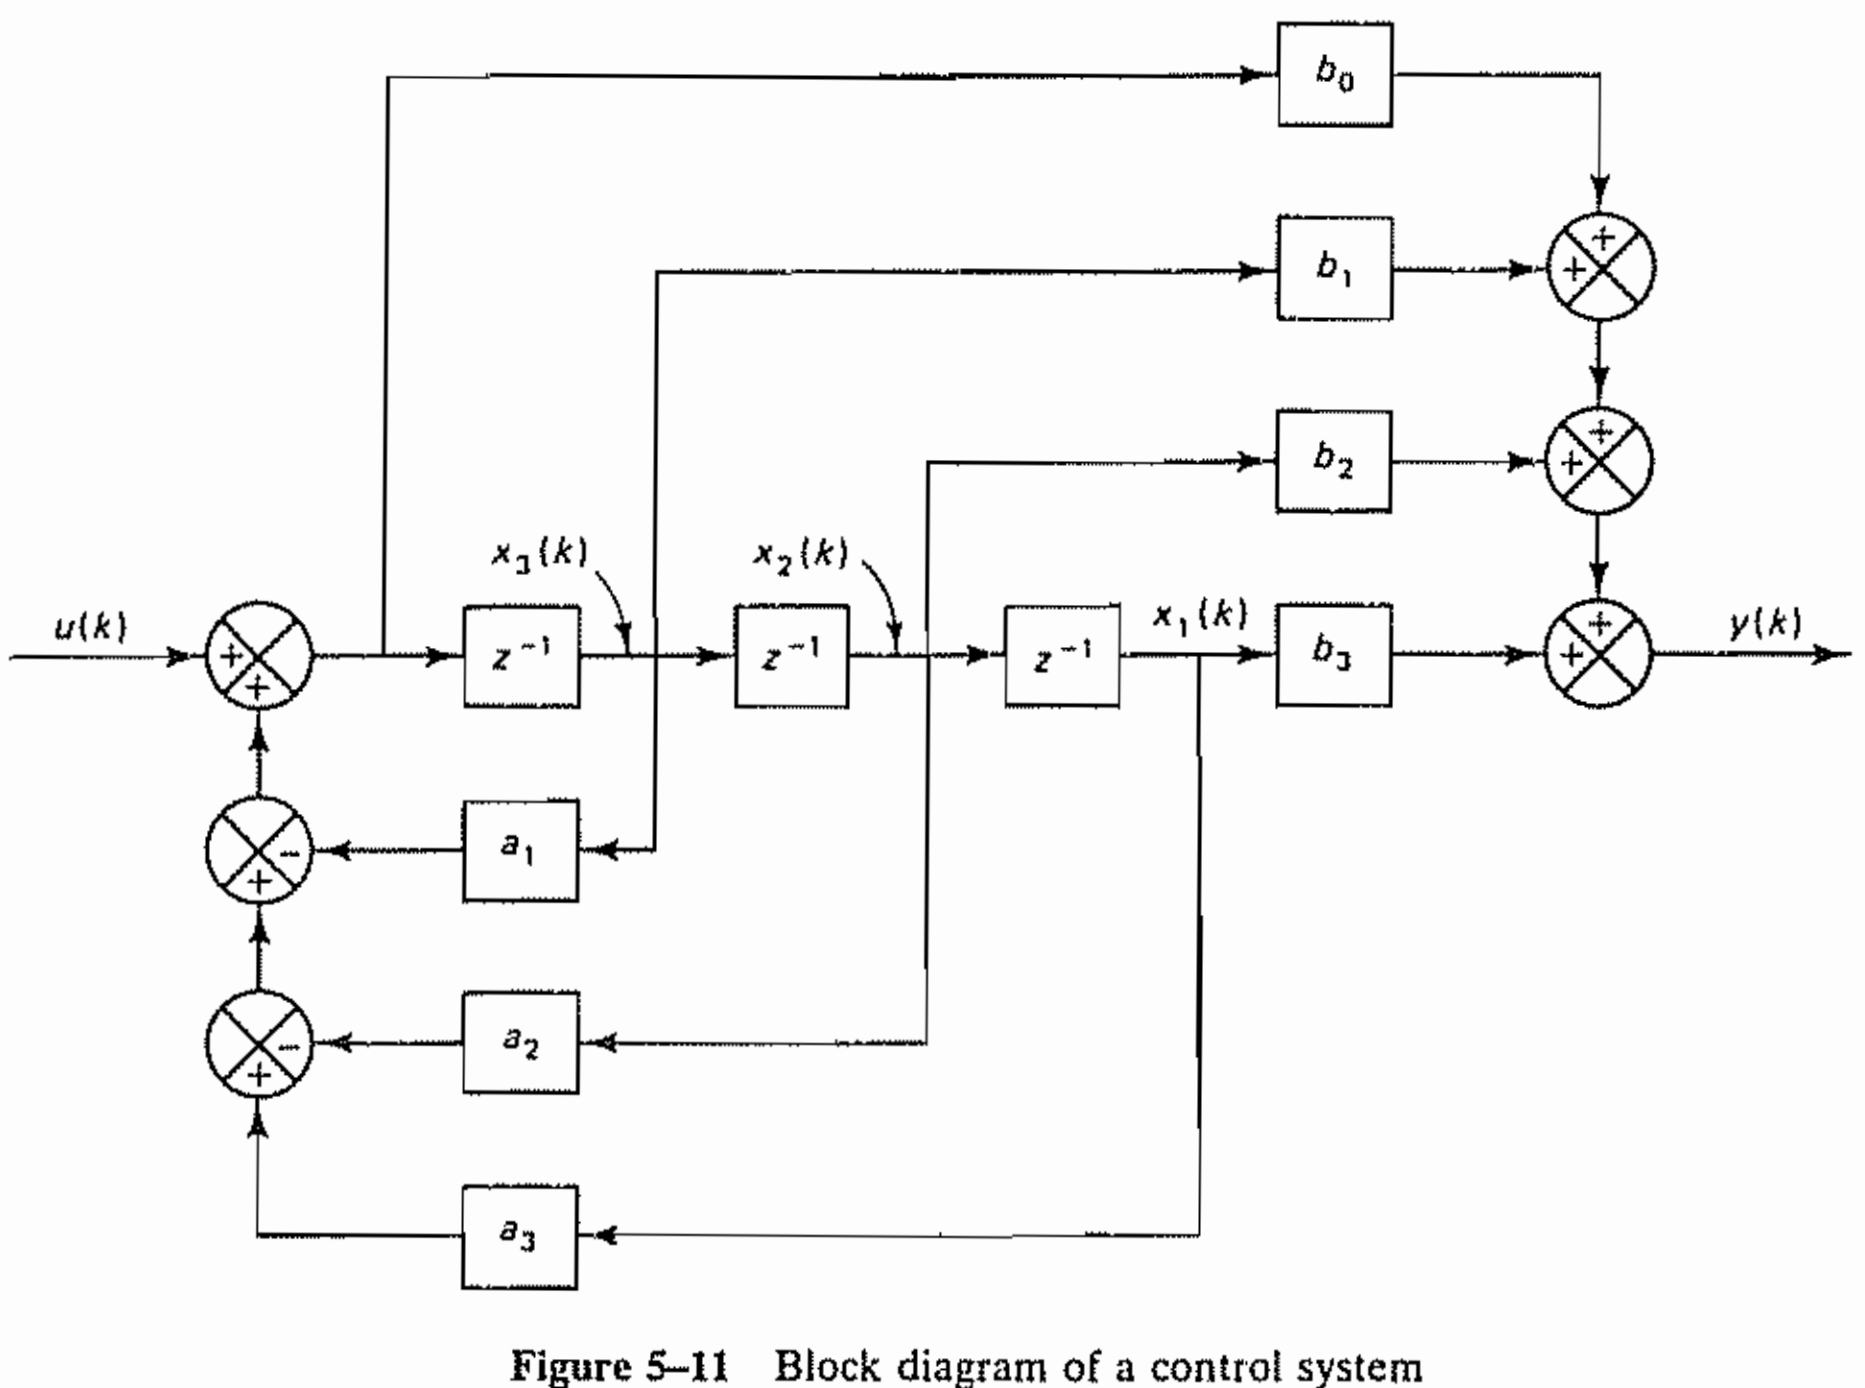
\includegraphics[width=0.6\linewidth]{OgataB-5-5.png}
%	\caption{Block Diagram}
	\label{fig:ogatab-5-5}
\end{figure}

\begin{align*}
& \begin{bmatrix}
x_1(k+1) \\
x_2(k+1) \\
x_3(k+1)
\end{bmatrix}= \begin{bmatrix}
0   & 1    & 0    \\
0   & 0    & 1    \\
a_3 & -a_2 & -a_1
\end{bmatrix}\begin{bmatrix}
x_1(k) \\
x_2(k) \\
x_3(k)
\end{bmatrix}+ \begin{bmatrix}
0 \\
0 \\
1
\end{bmatrix} u(k) \\
& y(k) = \begin{bmatrix} b_3+a_3b_0
	& b_2 -a_2b_0 & b_1 -a_1b_0 
 \end{bmatrix}\begin{bmatrix}
 x_1(k) \\
 x_2(k) \\
 x_3(k)
 \end{bmatrix} + b_0 u(k)
\end{align*}
\subsubsection*{Problem B-5-8}
Figure 5-14 shows a block diagram of a discrete-time multiple-input-multiple-output system. Obtain state-space equations for the system by considering $x_1(k)$, $x_2(k)$, and $x_3(k)$ as shown in the diagram to be state variables. Then define new state variables such that the state matrix becomes a diagonal matrix.

\begin{figure}[H]
	\centering
	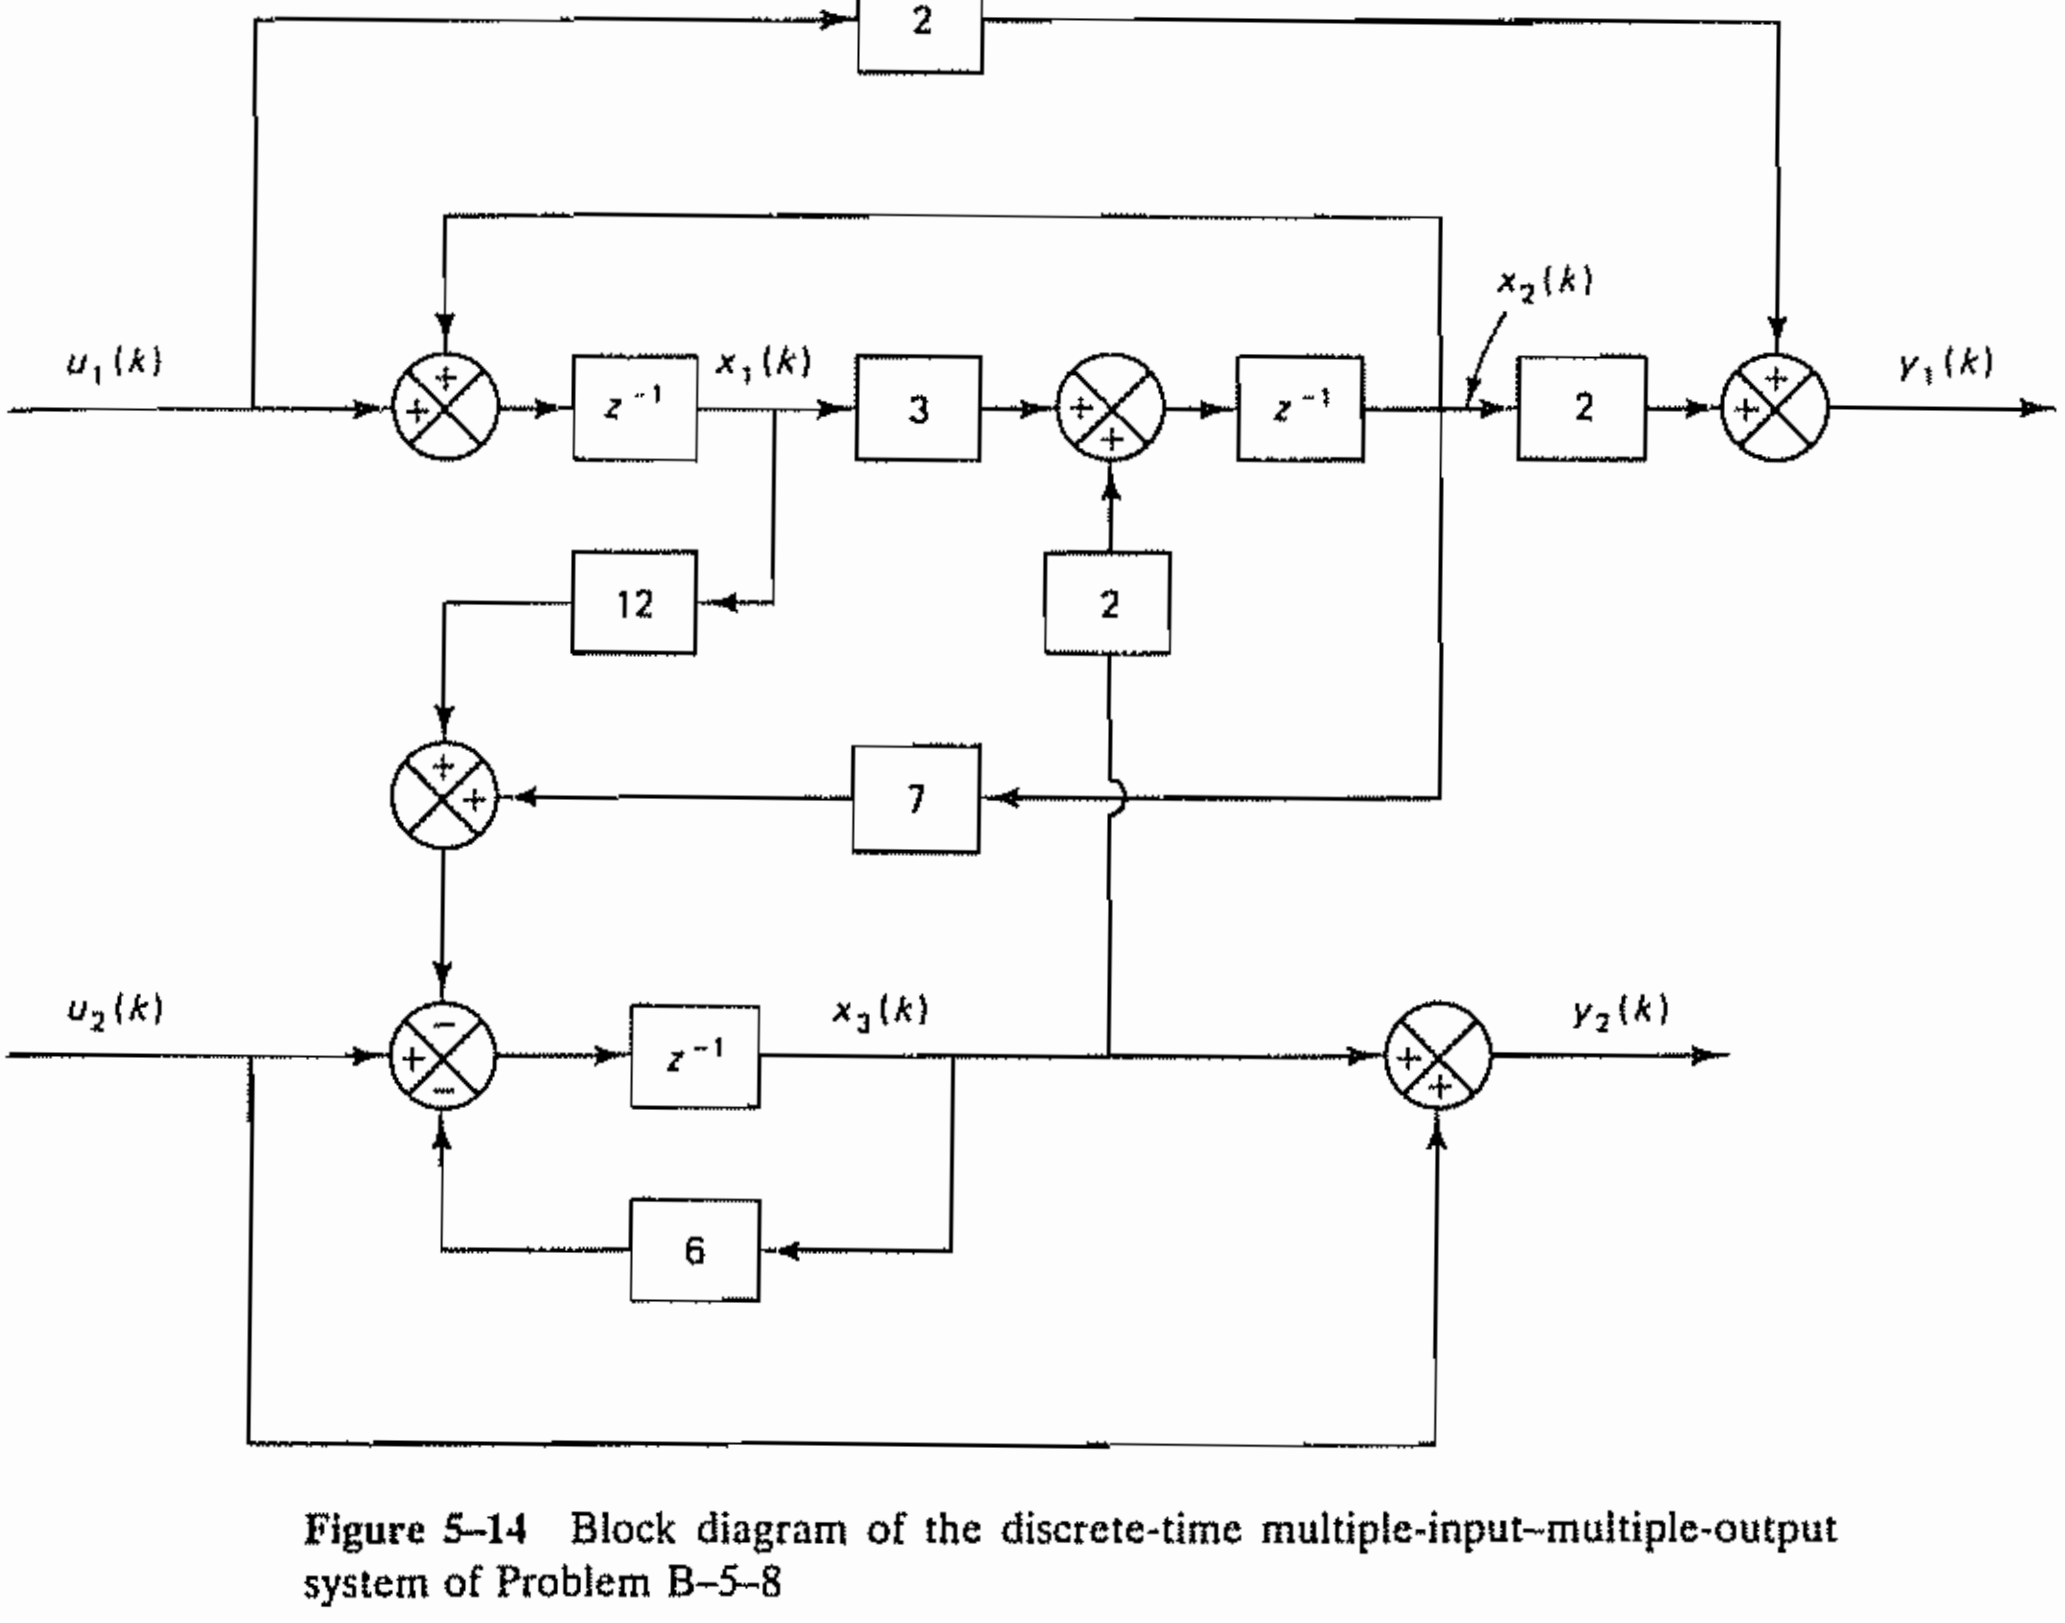
\includegraphics[width=0.6\linewidth]{OgataB-5-8.png}
	%	\caption{Block Diagram}
	%\label{fig:ogatab-5-5}
\end{figure}

\begin{align*}
& x_1(k+1)= x_2(k)+u_1(k) \\
& x_2(k+1)=3x_1(k)+2x_3(k) \\
& x_3(k+1)=-12x_1(k)-7x_2(k)-6x_3(k)+u_2(k) \\
& y_1(k)=2x_2(k)+2u_1(k) \\
& y_2(k)=x_3(k)+u_2(k)
\end{align*}

Rewriting the equations in state-space.

\begin{align*}
& \begin{bmatrix}
x_1(k+1) \
x_2(k+1) \\
x_3(k+1)
\end{bmatrix} = \begin{bmatrix}
0   &  1 & 0 \\
3   &  0 & 2 \\
-12 & -7 & -6
\end{bmatrix}\begin{bmatrix}
x_1(k) \\
x_2(k) \\
x_3(k)
\end{bmatrix}+\begin{bmatrix}
1   &  0 \\
0   &  0 \\
0   &  1
\end{bmatrix}\begin{bmatrix}
u_1(k)  \\  u_2(k)
\end{bmatrix} \\
& \begin{bmatrix}
y_1(k) \\ y_2(k)
\end{bmatrix} =\begin{bmatrix}
0   &  2  & 0 \\
0   &  0  & 1
\end{bmatrix}\begin{bmatrix}
x_1(k) \\
x_2(k) \\
x_3(k)
\end{bmatrix}+
\begin{bmatrix}
2 & 0 \\
0 & 1
\end{bmatrix}\begin{bmatrix}
u_1(k) \\
u_2(k)
\end{bmatrix}
\end{align*}
\subsubsection*{Problem B-5-15}
Obtain the pulse transfer function of the system defined by the equations

\begin{align*}
\quad x(k+1) & = Gx(k)+Hu(k) \\
\quad y(k)   & = Cx(k)+Du(k) \\
 & G = \begin{bmatrix}
-a_1 & -a_2 & -a_3 \\
1    &  0   &   0  \\
0    &  1   &   0
\end{bmatrix}, H = \begin{bmatrix}
1 \\ 0 \\ 0
\end{bmatrix} \\
& C = [b_1-a_1 \quad   b_2 - a_2b_0 \quad  b_3 - a_3b_0], D= b_0
\end{align*}

\begin{align*}
& \textrm{let } M =\begin{pmatrix}a&b&c\\ d&e&f\\ g&h&i \end{pmatrix} \\
& M^{-1}=\frac{1}{a(ei-fh) - b(di-fg) + c(dh-eg)}  \begin{pmatrix} ei-fh&ch-bi&bf-ce\\ fg-di&ai-cg&cd-af\\ dh-eg&bg-ah&ae-bd \end{pmatrix} \\
& (zI-G)^{-1}= \begin{bmatrix}
z+a_1 & a_2 & a_3 \\
-1    & z   & 0   \\
0     & -1  & z 
\end{bmatrix}^{-1} = \frac{1}{z^3+a_1z^2+a_2z+a_3} \begin{bmatrix}
z^2 & -(a_2z+a_3) & -a_3 z \\
z   & z^2+a_1z    &  -a_3  \\
1   & z+a_1       & z^2+a_1z +a_2
\end{bmatrix} \\
& (zI-G)^{-1}H= \begin{bmatrix}
z^2 & -(a_2z+a_3) & -a_3 z \\
z   & z^2+a_1z    &  -a_3  \\
1   & z+a_1       & z^2+a_1z +a_2
\end{bmatrix}\begin{bmatrix}
1 \\ 0 \\ 0
\end{bmatrix} = \frac{1}{z^3+a_1z^2+a_2z+a_3} \begin{bmatrix}
z^2  \\
z    \\
1   
\end{bmatrix} \\
& C(zI-G)^{-1}H = [b_1-a_1 \quad   b_2 - a_2b_0 \quad  b_3 - a_3b_0]\frac{1}{z^3+a_1z^2+a_2z+a_3} \begin{bmatrix}
z^2  \\
z    \\
1   
\end{bmatrix} \\
& F(z) = C(zI-G)^{-1}H +D =  \frac{(b_1-a_1b_0)z^2 + (b_2 - a_2b_0)z (b_3 - a_3b_0)}{z^3+a_1z^2+a_2z+a_3} + b_0 \\
& F(z)= \frac{b_0z^3+b_1z^2+b_2z+b_3}{z^3+a_1z^2+a_2z+a_3}
\end{align*}